% XeLaTeX can use any Mac OS X font. See the setromanfont command below.
% Input to XeLaTeX is full Unicode, so Unicode characters can be typed directly into the source.

% The next lines tell TeXShop to typeset with xelatex, and to open and save the source with Unicode encoding.

%!TEX TS-program = xelatex
%!TEX encoding = UTF-8 Unicode

\documentclass{article}
\usepackage[utf8]{inputenc}    % si besoin

\usepackage{amsmath,amssymb}   % si vous utilisez des formules avancées

\usepackage{tikz}       % TikZ "de base"
\usepackage{pgfplots}   % Pour les tracés pgfplots
\pgfplotsset{compat=1.18} % ou version plus récente, p. ex. 1.18

\begin{document}



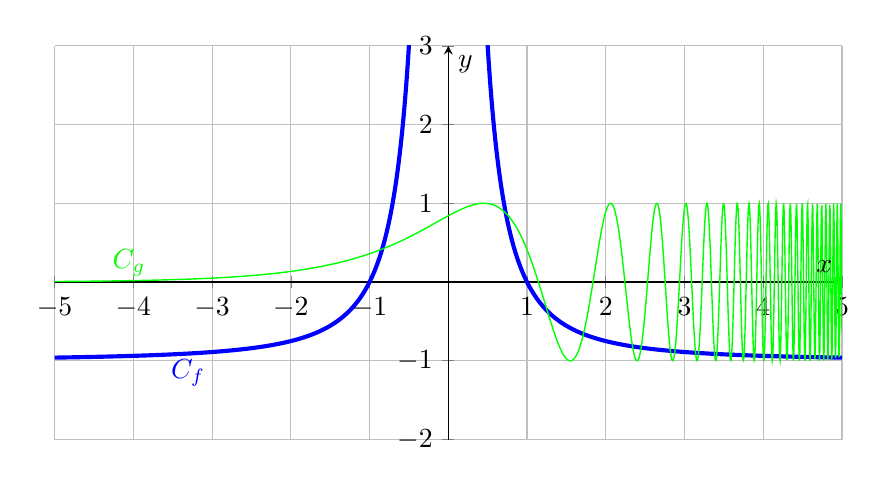
\begin{tikzpicture}
  \begin{axis}[%
    xmin=-5.0,
    xmax=5.0,
    ymin=-2.0,
    ymax=3.0,
    axis lines=middle,
    trig format=rad,
    grid=major,
    xtick distance=1.0,
    ytick distance=1.0,
    xlabel=$x$,
    ylabel=$y$,
    scale only axis,
    x=1.0cm,
    y=1.0cm
  ]
    \addplot[samples=2000, unbounded coords=jump, line width=1.5pt, color=blue, solid, restrict y to domain=-100.0:100.0, domain=-5.0:5.0]{-1 + x^(-2)};
    \draw[color=blue] (axis cs:-3.645161290322581,-1.1533466533466534) node[anchor=west]{\color{blue}$C_f$};
    \addplot[samples=2000, unbounded coords=jump, line width=0.5pt, color=green, solid, restrict y to domain=-100.0:100.0, domain=-5.0:5.0]{sin(exp(x))};
    \draw[color=green] (axis cs:-3.722580645161291,0.23811902383330974) node[anchor=east]{\color{green}$C_g$};
  \end{axis}
\end{tikzpicture}

\end{document}  